\chapter{Proposed Semi-Automatic Evaluation Method}

The method we propose consists of two parts. The first part is a way how humans
judge outputs of judged systems. The second part is how to interpret collected
judgments to compute overall scores and rank the systems. We discuss these two
parts in following two sections. \XXX{V tomto odstavci (a asi i v dalsich odstavcich
neni dostatecne zdurazneno, proc je to semi-automaticka metoda, mozna opustit
oznaceni semi-automaticka a pouzit misto toho neco jako Manual Evaluation Method
with posibility to reuse collected judgementes for new systems)}

In the WMT official human evaluation humans judge whole sentences. They get
five candidate translations of a given source sentence and their task is to
rank these candidates relatively (ties are allowed). One of disadvantages of
this method is that sentences are quite long and therefore quite hard to
remember for judge to compare them. Also when comparing longer sentences there
are much more aspects in which one sentence can be better or worse than second
sentence and therefore it is more difficult for judges to choose the better
candidate. 

%\begin{algorithm}[H]
%    \KwData{Tree, MaxSegmentLength}
%    \KwResult{List of extracted segments}
%    \If{Tree covers more than MaxSegmentLength}{
%      yield all leaves \;
%    }
%    \caption{Segment extraction from parsed tree}
%    \label{segment:extraction}
%\end{algorithm}

To avoid these disadvantages we propose the following method. Instead of
judging whole sentences we extract shorter segments from candidates and give
them to judges to rank them. In order to extract meaningful segments with the
same meaning from all candidates we do the following procedure: First we parse
the source sentence and then we go recursively down the parsed tree and find
nodes which covers source segments with given maximum length (which is a
parameter of this method). This is exactly described in algorithm
\ref{segment:extraction}. Finally we project these extracted source segments to
their counterpart segments in all candidate sentences using an automatic
alignment.  You can find the whole process ilustrated in figure \XXX{nakreslit
obrazek}.  This extraction method is inspired by \XXX{citovat ten clanek a
stary WMT clanek}.

In \XXX{citovat WMT}, these extracted segments are only highlighted and shown
to judges together with the rest of the sentence. Judges are asked to rank the
segments in the context of whole sentences. \XXX{Zkontrolovat presne instrukce
z WMT}

We use different approach here which is more similar to that used in
\XXX{citovat ten clanek}. We show the extracted segments without any context
and ask judges to rank them. The only additional information provided to
annotators is the whole source sentence with the source segment highlighted.
Judges are told that they can imagine the rest of the sentence in which the
ranked segment fits best. They are instructed to penalize only those segments
for which they cannot imagine any appropriate rest of the sentence.

While we are aware that this approach has some disadvantages (which we
summarize bellow) there is one significant advantage: it is much more likely
that two systems produce the same translation of a short segment then they
would produce the same translation of a whole sentence. Because we do not show
the sentence context to annotators we can merge the equal segment candidates
into one, so the annotators have less candidate segments to rank. This also
allows us to reuse already collected human judgements later to evaluate a new
system which was not in the set of annotated systems (we present this
experiment in the section \ref{evaluating-new-systems}) or to tune parameters
of a system (we present this experiment in the section \ref{tuning-systems}).

\section{Data and Segment Preparation}

We have conducted an annotation experiment using the proposed method. In this
section we describe what data we have used and how we prepare them for the
annotation experiment.

We used English to Czech part of the WMT14 \parcite{wmt14-overview-paper} test
set. We choose this data set to be able to compare experiments' results with
the official WMT14 human evaluation. 

The testset consists of 3003 sentences (68866 tokens). It contains both source
sentences and reference translations. Roughly a half of the sentences was
originally in Czech and was translated by human translators into English. The
second half of the sentences was translated in opposite direction. Besides the
source and reference translations, we also used candidate translations of 10
systems which participated in the WMT14 translation task. All systems are
listed in the table \ref{translation-task-participants}


\begin{table}[h]
  \small
  \begin{center}
    \begin{tabular}{|l|l|l|}
      \hline
      \textbf{ID} & \textbf{Type} & \textbf{Team} \\
      \hline
      \system{cu-depfix} & statistical & \multirow{4}{*}{Charles University, Prague \XXX{(Tamchyna et al., 2014)}}  \\
      \system{cu-bojar} & statistical &  \\
      \system{cu-funky} & statistical &  \\
      \system{cu-tecto} & statistical &  \\
      \hline
      \system{uedin-phrase} & statistical &  \multirow{2}{*}{University of Edinburgh \XXX{(Durrani er al., 2014b)}} \\
      \system{uedin-uncnstr} &  statistical &  \\
      \hline
      \system{commercial-1} & rule-based & \multirow{2}{*}{Commercial machine translation systems} \\
      \system{commercial-2} & rule-based & \\
      \hline
      \system{online-a} & statistical & \multirow{2}{*}{Online statistical machine translation systems} \\
      \system{online-b} & statistical & \\
      \hline
    \end{tabular}
  \end{center}
  \caption{Systems participating WMT14 translation task in direction English-Czech \XXX{Zkontrolovat typy nekterych systemu}}
  \label{translation-task-participants}
\end{table}

Source sentences and all candidate translations were tokenized using the script
\script{tokenizer.perl}. Unicode punctuation characters were normalized using
the script \script{replace-unicode-punctuation.perl}. (Both scripts are included
in the Moses toolkit).

The source sentences were parsed using the Stanford lexicalized parser
\XXX{citace}. We used \pojem{englishFactored} model which is distributed with
the parser. (More models were examined and this model gave subjectively the
best segments). \XXX{Tady popsat detailneji, ktere modely jsem zkusil a ze 
to nebylo zase tak subjektivni}

We computed an alignments between the source sentecnes and the candidate
translations using Giza++ \XXX{citace}. Since the alignment algorithm is
unsupervised and the amount of all candidate translations is relatively small
($10 \times 3003$), we introduced more data by concatenating all candidate
translations with Europarl parallel corpus (646 605 sentences, \XXX{citovat})
and with \XXX{Jaky je to korpus?} (197 053 sentences, \XXX{citovat}).  The
concatenated parallel corpus was lowercased before alignment computation. 

We extracted short segments from the parsed source trees using the algorithm
\ref{segment:extraction}. The constant \pojem{min-segment-length} was set to
the value 3 to filter out very short segments which are hard to judge without
context. This also helped to reduce the number of extracted segments to be
annotated. The constant \pojem{max-segment-length} was set to the value 6 so
the extracted segments were not too long to judge and in the same time it was
more likely that two candidate translations of a segment were equal and
therefore there would be less items to rank (our aim was to make annotations as
easy and fast as possible). We have experimented with various settings of these
two constants and the final settings seemed to generate reasonable number of
meaningful segments.

\XXX{Nekde zduraznit, ze to jsou vlastne konstituenty, ale asi ne tady, nekde drive}

From 3003 source sentences, we have extracted 8485 segments of length 3 to 6
tokens. That is \XXX{priblizne} 2.83 segments on a sentence on average. By
projecting the source segments to the candidate sentences using the computed
alignments, we got $10 \times 8485 = 84850$ candidate segments. However, after
the merging of equal segments only 50011 candidate segments left. This is 58.9
\% of the original candidate segments, or in other words, after the merging we
got 5.89 (instead of original 10) candidate segments to be ranked for each
source segment on average. Theese prepared candidate segments were inserted
into the database to be ranked by annotators.

\section{Segments Ranking}

We have developed a new annotation application for this annotation
project.\footnote{It would be probably possible to customize and use an
    existing annotation application, for example Appraise\XXX{citovat}.
    However, since the ranking of short segments is quite specific it would
require a lot of customization. We therefore decided to develop our own
light-weight web application which would suit our needs perfectly and allow us
to optimize efficiency of the annotation.} For implementation details of this
application, please see the chapter \ref{implementation}.

You can find an example screen shot of this application in figure
\ref{segranks-screenshot}. Annotation instructions were displayed on each
annotation screen. This is an English translation of these instructions:

\begin{quote}
A number of segments are extracted from the annotated sentence. You are shown a
few candidate translations for each of these segments. Your task is to
distinguish the acceptable candidate translations (the meaning of the segment
can be guessed despite a few or more errors) from the unacceptable ones (the
meaning is definitely not possible to guess from the candidate segment). Also
please rank the acceptable candidate translations relatively from the best ones
to the worst ones.  Please, place better candidate translations higher, the
worser ones lower. You can place candidates of the same quality on the same
rank. Please place the unacceptable candidates to the position ``Garbage''

Please note that source segments and their candidate translations are chosen
automatically and does not have to be perfect. Consider them as only
approximate clue. If a candidate segment contains an extra word, which does not
correspond to the source segment but otherwise could be in the translated
sentence you do not have to consider such candidate as worser. If something is
missing in the candidate translation you should consider that as an error.
\end{quote}

Our goal was to make the annotation as efficient and user friendly as possible.
Annotators rank all the source segments of a sentence on a single screen (so
that they have to read the whole source sentence and reference translation only
once). For each annotated segment they see the source sentence repeated with
the annotated segment highlighted. Annotators rank the segment candidates by
drag-and-droping them to appropriate rank positions. When all candidates of all
source segments of a sentence are ranked annotators are allowed to submit the
results to the server.

The web interface has responsive design, so it works correctly on mobile
devices.  The drag-and-drop works also on touch screens. Annotators were
therefore able to rank segments on a tablet.



\begin{figure}
    \begin{center}
        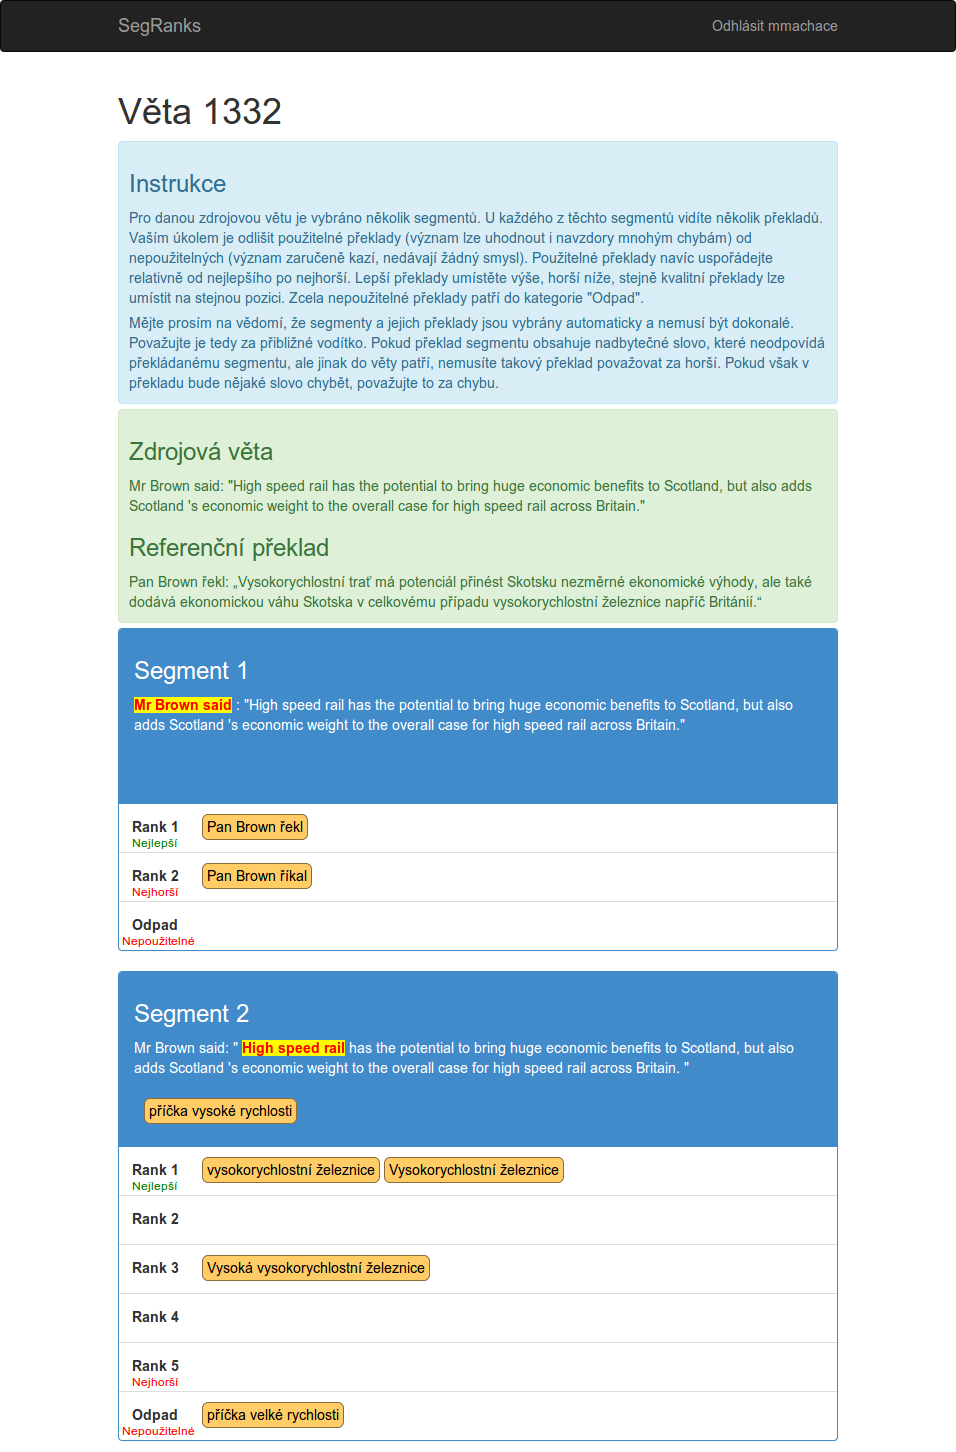
\includegraphics[width=\textwidth]{img/segranks-screenshot2.png}
    \end{center}
    \caption{A screenshot of an annotation application. Annotators rank the
    candidate segments by draging and dropping them into the ranks.
Annotators see all annotated segments of a sentence on single screen}
    \label{segranks-screenshot}
\end{figure}


\XXX{zduraznit jednoduchost,
anotatori,  prubeh anotace, statistiky analyza
ziskane databaze, mezianotatorske shody, cena, platby}

\XXX{Je vubec slovo segment vhodne??? Span?? Constituent??}


\section{Experiments}

\subsection{Evaluating Annotated Systems}
\XXX{Zde uvedu vzorecek (mozna vice variant) pro vypocet skore systemu, ktere
byly anotovane. Vypocet skore, vypocet korelace s oficialnimi WMT14 vysledky.
Porovnani obou metod z hlediska mnozstvi lidske prace.}

\subsection{Evaluating New Systems}
\label{evaluating-new-systems}

\XXX{Zde zkusim pouzit vytvorenou databazi pro vyhodnoceni noveho systemu}

\XXX{provest experimenty podobne tem z clanku An Evaluation Tool for Machine
Translation: Fast Evaluation for MT Research}

\subsection{Tuning Systems}
\label{tuning-systems}

\XXX{Zde zkusim pouzit vytvorenou databazi pro MT tuning}

\section{Comparison to Other Manual Methods}
